The natural generalization of MPS to higher dimensional lattices is given by \textit{Projected Entangled Pair States} (PEPS) \cite{cite:algorithms_for_finite_PEPS, cite:mps_and_peps_concepts_symmetries_theorems}. A PEPS is constructed similar to an MPS by representing the local subsystem on each lattice site $j$ with the index $i_j$ of a tensor $T^{[j],i_j}$ and connecting nearest-neighbour tensors with virtual bonds. The maximum bond dimension of virtual bonds is called $D$ and controls both the representational power of the PEPS and the computational cost of algorithms. The full quantum state can be written as
\begin{equation}
	\label{eq:PEPS_definition_general}
	\ket{\Psi} = \sum_{i_1,i_2,\dots,i_N} \mathcal{C}\left(T^{[1],i_1}, T^{[2],i_2}, \dots, T^{[N],i_N}\right) \ket{i_1,i_2,\dots,i_N},
\end{equation}
where $\mathcal{C}(\dots)$ denotes the contraction of the full network along all virtual bonds. As an example, we draw a PEPS on a square lattice in Figure \figref{fig:square_PEPS}. \par
\begin{figure}
	\centering
	\subcaptionbox{\label{fig:square_PEPS}}
	{%
		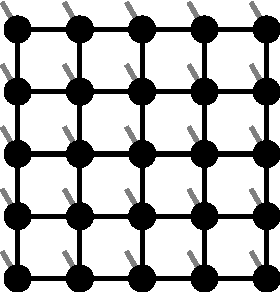
\includegraphics[scale=1]{figures/tikz/Tensor_Networks/isoTPS_structure/isoTPS_structure_a.pdf}
	}
	\quad\quad
	\subcaptionbox{\label{fig:square_isoTPS}}
	{%
		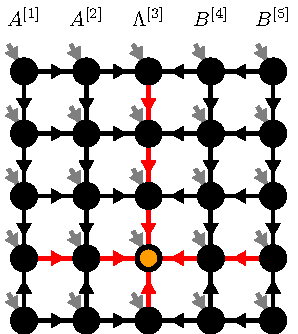
\includegraphics[scale=1]{figures/tikz/Tensor_Networks/isoTPS_structure/isoTPS_structure_b.pdf}
	}
	\caption{Tensor Networks representing two dimensional quantum states on a square lattice. (a) A Projected Entangled Pair State (PEPS). (b) An isometric Tensor Product State (isoTPS). The orthogonality hypersurface is drawn in red and the orthogonality center in orange.}
	\label{fig:square_PEPS_and_isoTPS}
\end{figure}
PEPS are able to efficiently represent area law states in two and higher dimensions \cite{cite:practical_introduction_MPS_and_PEPS}. Remarkably, PEPS can even represent certain states with correlations decaying polynomially with separation distance \cite{cite:criticality_the_area_law_and_the_computational_power_of_PEPS}, whereas MPS can only handle exponentially decaying correlations. Polynomially decaying correlations are characteristic for critical points. \par
Unfortunately, it is not generally possible to bring a PEPS into an exact canonical form due to the presence of closed loops. Because of this, already the computation of local expectation values scales exponentially with system size and can only be computed approximately in practice, e.g., using the boundary MPS method \cite{cite:practical_introduction_MPS_and_PEPS} or corner transfer matrices \cite{cite:CTMRG}. Moreover, algorithms for ground state search and time evolution have computational costs scaling with high powers of the bond dimension. For example, the cost of a full update TEBD iteration is dominated by the contraction of an effective environment, scaling as $\mathcal{O}\left(D^{10}\right)$ \cite{cite:unifying_PEPS_contractions}. \par
Recently, the new class of \textit{isometric Tensor Product States} (isoTPS) has been introduced \cite{cite:isometric_tensor_network_states_in_two_dimensions, cite:conversion_of_PEPS_into_a_canonical_form, cite:DMRG_approach_to_optimizing_2D_tensor_networks}, generalizing the canonical form of MPS to higher dimensions by enforcing isometry constraints. In the following, we will give a brief introduction to the isoTPS defined in \cite{cite:isometric_tensor_network_states_in_two_dimensions}. A two-dimensional isoTPS on the square lattice is constructed by enforcing the isometry conditions shown in Figure \figref{fig:square_isoTPS}. The isometries are chosen in such a way that all arrows point towards a special row and column, called the \textit{orthogonality hypersurface} of the isoTPS. The term \textit{hypersurface} is chosen in anticipation of a generalization to higher dimensions. The maximum bond dimension of bonds along the orthogonality hypersurface is increased to $\chi = f\cdot D$, where $f \ge 1$ is a positive integer. In practice, this can produce better results at similar computational costs than increasing the maximum bond dimension for all bonds of the lattice \cite{cite:efficient_simulation_of_dynamics_in_two_dimensional_quantum_spin_systems}. \par
Because of the isometry condition, one can think of the contractions of each of the four regions outside the orthogonality hypersurface as orthogonal boundary maps \cite{cite:efficient_simulation_of_dynamics_in_two_dimensional_quantum_spin_systems}. The single tensor with only incoming arrows is called the \textit{orthogonality center}. Local expectation values of operators acting in the vicinity of the orthogonality center can be computed efficiently because most contractions reduce to identity, similar to the computation of local expectation values in MPS. The orthogonality center can be moved along the orthogonality hypersurface simply and exactly using a QR-decomposition as shown in Figure \figref{fig:isoTPS_moving_ortho_center}.\par
\begin{figure}
	\centering
	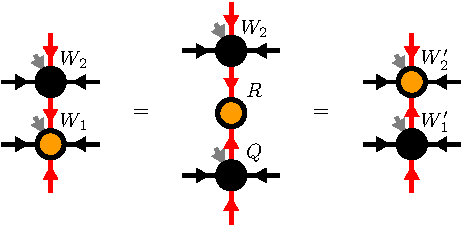
\includegraphics[scale=1]{figures/tikz/Tensor_Networks/isoTPS_moving_ortho_center/isoTPS_moving_ortho_center.pdf}
	\caption{Moving the orthogonality center along the orthogonality hypersurface can be done easily via a single QR-decomposition. First, the orthogonality center is split as $W_1 = QR = W_1^\prime R$. The tensors $W_2$ and $R$ are then contracted to form the new orthogonality center $W_2^\prime$}
	\label{fig:isoTPS_moving_ortho_center}
\end{figure}
\begin{figure}
	\centering
	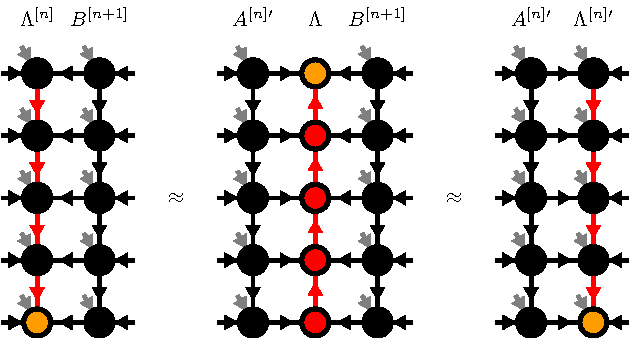
\includegraphics[scale=1]{figures/tikz/Tensor_Networks/isoTPS_moving_ortho_surface/isoTPS_moving_ortho_surface.pdf}
	\caption{The orthogonality hypersurface can be moved to the right by first solving Equation \eqref{eq:isoTPS_moving_ortho_surface_auxillary_formulation} variationally and then absorbing $\Lambda$ into $B^{[n+1]}$ via the standard MPO-MPS multiplication and MPS compression algorithms.}
	\label{fig:isoTPS_moving_ortho_column}
\end{figure}
Moving the orthogonality surface is a harder problem, which can in general only be done approximately. In analogy to MPS and as shown in Figure \figref{fig:square_isoTPS}, we call columns left of the orthogonality hypersurface $A^{[n]}$ and columns right of the orthogonality hypersurface $B^{[n]}$, with $n = 1,2,\dots,L$ and $L$ the linear system size. Moving the orthogonality hypersurface $\Lambda^{[n]}$ one column to the right can be expressed as solving the problem
\begin{equation}
	\label{eq:isoTPS_moving_ortho_surface_general}
	\Lambda^{[n]} B^{[n+1]} \approx A^{[n]} \Lambda^{[n+1]},
\end{equation}
where the notation $\Lambda^{[n]} B^{[n+1]}$ denotes the contraction of columns $\Lambda^{[n]}$ and $B^{[n+1]}$ along their connecting bonds. Instead of \eqref{eq:isoTPS_moving_ortho_surface_general}, one can solve the simpler auxiliary problem
\begin{equation}
	\label{eq:isoTPS_moving_ortho_surface_auxillary_formulation}
	\Lambda^{[n]} = A^{[n]} \Lambda,
\end{equation}
where $\Lambda$ is a column of tensors with no physical indices, as shown in Figure \figref{fig:isoTPS_moving_ortho_column}. This column can then be absorbed into $B^{[n+1]}$ via the standard algorithm of applying a Matrix Product Operate (MPO) to an MPS and subsequently compressing the MPS to the maximal bond dimension \cite{cite:DMRG_in_the_age_of_MPS} to form the new orthogonality hypersurface $\Lambda^{[n+1]}$. One can variationally solve problem \eqref{eq:isoTPS_moving_ortho_surface_auxillary_formulation} by minimizing the distance $\left\lvert\Lambda^{[n]}-A^{[n]}\Lambda\right\rvert$, sweeping over all tensors of the columns $A^{[n]}$ and $\Lambda$ and performing local optimizations while respecting the isometry condition. This is known as an Evenbly-Vidal style variational optimization and is discussed in more detail in Appendix \ref{app:optimization_problems_for_isometric_tensor_networks}.
\begin{figure}
	\centering
	\subcaptionbox{\label{fig:Moses_move}}
	{%
		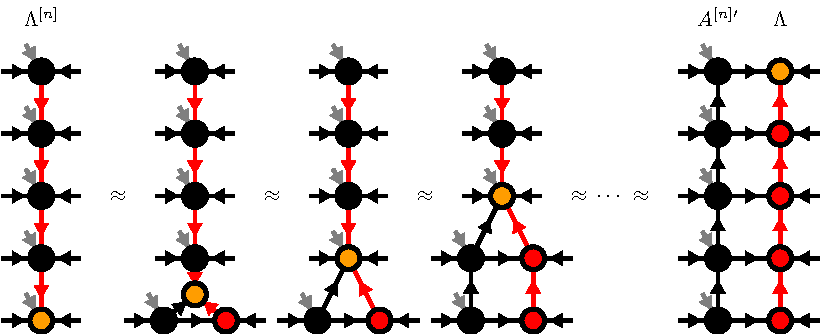
\includegraphics[scale=1]{figures/tikz/Tensor_Networks/isoTPS_MM/isoTPS_MM_a.pdf}
	}
	\par\medskip
	\subcaptionbox{\label{fig:tripartite_decomposition}}
	{%
		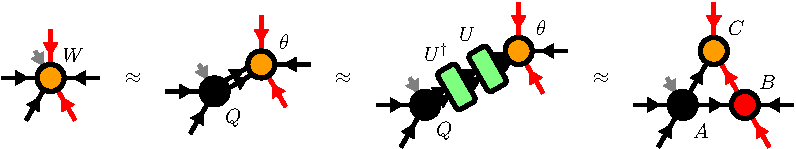
\includegraphics[scale=1]{figures/tikz/Tensor_Networks/isoTPS_MM/isoTPS_MM_b.pdf}
		
	}
	\caption{(a) The Moses Move (MM) splits the column $\Lambda^{[n]}$ into $A^{[n]}$ and $\Lambda$ via a single unzipping sweep of tripartite decompositions. (b) Tripartite decomposition of the tensor $W$ as explained in the text.}
	\label{fig:Moses_move_and_tripartite_decomposition}
\end{figure}
It is however found in \cite{cite:isometric_tensor_network_states_in_two_dimensions} that a single unzipping sweep, called the \textit{Moses Move} (MM), provides a solution very close to the variational one whilst being far quicker. The MM can also be used as a good initialization for the variational algorithm. We sketch the MM in Figure \figref{fig:Moses_move}. Starting from the bottom of the orthogonality hypersurface column, the tensors are split one after the other using tripartite decompositions. A single tripartite decomposition of a tensor $W$ is shown in Figure \figref{fig:tripartite_decomposition}. First, $W$ is split into two tensors $Q$ and $\theta$ via a truncated SVD $W = U(SV) = Q\theta$, where $Q$ is an isometry. The bond connecting $Q$ and $\theta$ is then reshaped into two bonds of bond dimension $<D$. Next, it is important to note that the full contraction is invariant under the insertion of a unitary $U$ and its conjugate transpose, $Q\theta = (QU^\dagger)(U\theta)$, with $A = QU^\dagger$ still satisfying the isometry condition. This degree of freedom can be used to \textit{disentangle} the tensor $\theta$ along the vertical direction. Accordingly, we choose $U$ such that the truncation error or some entanglement measure is minimized for splits of $\theta$ along this direction. Choosing a good disentangling unitary is crucial for a successful tripartite decomposition and will be discussed further in Section \ref{sec:YB_isoTPS_yang_baxter_move}. Assume for now that a good disentangling unitary has been found. After contracting $QU^\dagger$ and $U\theta$, a truncated SVD is used to split $U\theta$ into tensors $B$ and $C$ as shown in Figure \figref{fig:tripartite_decomposition}, completing the tripartite decomposition. The computational cost of the MM scales with the maximum bond dimension $D$ as $\mathcal{O}(D^7)$ \cite{cite:isometric_tensor_network_states_in_two_dimensions, cite:efficient_simulation_of_dynamics_in_two_dimensional_quantum_spin_systems}.\par
Because the orthogonality center can be moved easily along the orthogonality hypersurface, one can think of the orthogonality hypersurface along a column or row as a 1D MPS with an enlarged physical bond dimension grouping together the physical and the two auxiliary legs protruding from the orthogonality hypersurface tensors. Standard MPS algorithms can then be generalized to isoTPS by performing one iteration of the algorithm on the orthogonality hypersurface MPS, before moving the hypersurface via the MM and repeating the procedure. As an example, we will discuss TEBD$^2$, the generalization of TEBD to an isoTPS on a 2D square lattice. The Hamiltonian $\hat{H}$ is first split into terms acting on columns and rows,
\begin{equation}
	\hat{H} = \sum_{x = 1}^{L_x} \hat{H}_x + \sum_{y = 1}^{L_y} \hat{H}_y,
\end{equation}
and the time evolution operator is replaced by the first order approximation
\begin{equation}
	\hat{U}^\text{TEBD1}(\Delta t) = \prod_{y=1}^{L_y} e^{-i\Delta t\hat{H}_y} \prod_{x=1}^{L_x} e^{-i\Delta t\hat{H}_x} .
\end{equation}
If the orthogonality hypersurface $\Lambda^{[x]}$ is at column $x$, the operator $e^{-i\Delta t\hat{H}_x}$ can easily be applied by calling the standard 1D TEBD algorithm at a cost of $\mathcal{O}(D^6)$ \cite{cite:isometric_tensor_network_states_in_two_dimensions}. To evolve the full isoTPS, we start with the orthogonality center in the bottom left corner and apply first the time evolution operators along all columns, moving from left to right using the MM. We then rotate the lattice by $90^\circ$, turning rows into columns and columns into rows. Moving back from right to left we now apply the time evolution operators along the rows, completing the time step. \par
The computational cost of the full TEBD$^2$ algorithm scales as $\mathcal{O}(D^7)$. The algorithm can be easily improved to second order by symmetrizing the time evolution \cite{cite:efficient_simulation_of_dynamics_in_two_dimensional_quantum_spin_systems}.